\documentclass[a4paper,12pt]{article}
\usepackage{../../mypackages}
\usepackage{../../macros}


\usepackage{pgfplots}
    \pgfplotsset{
    compat=1.11,
  }

\setlength{\parindent}{0pt}


\begin{document}

\title{Chapitre 1 - Organisation et transformation de la matière}
\author{N. Bancel}

\maketitle

\section*{La masse volumique}

\subsection*{Utilité}
\begin{itemize}[noitemsep]
  \item Identification de la matière d'un objet
  \item Différienciation d'espères chimiques
  \item Détermination d'un volume complexe par sa masse 
\end{itemize}


\subsection*{Définitions}

\begin{tcolorbox}
La masse d'un corps représente la quantité de matière qui le compose. \par
\textbf{Remarque} : Elle est constante quelque soit l'endroit où l'on se trouve (sur Mars, sur Terre, sur la Lune) \par
\textbf{Unité} : Dans le système international, l'unité légale de la masse est le kilogramme (symbole \textbf{kg})

\end{tcolorbox}

\begin{tcolorbox}
  Le volume d'un corps est la grandeur qui indique l'espace qu'il occupe. \par
  \textbf{Unité} : Dans le système international, l'unité légale du volume est le mètre cube (symbole \textbf{$m^3$})
\end{tcolorbox}

Cela représente le volume d'un cube d'un mètre de côté.

\begin{tcolorbox}
  Le masse volumique est la masse de ce matériau par unité de volume \par
  \textbf{Unité} : Unité légale de la masse volumique est le kilogramme par mètre cube (symbole \textbf{$kg / m^3$})
\end{tcolorbox}

\subsection*{Relation entre masse, volume et masse volumique}

Pour un matériau \textbf{plein} donné, la masse et le volume sont proportionnels. 

\begin{tcolorbox}
  La relation de proportionnalité entre la masse m et la volume V du matériau s'écrit
  \(m = \rho * V\)
  Le coefficient de proportionnalité \(\rho\) est la masse volumique du matériau
\end{tcolorbox}



\subsection*{Détermination de la masse volumique d'un solide}

\textbf{Source} : \href{https://www.maxicours.com/se/cours/determiner-une-masse-volumique-experimentalement--seconde--physique-chimie/}{Maxicours - La masse volumique}

Etapes 
\begin{enumerate}[noitemsep, label=(\arabic*)]
  \item Déterminer le volume.
  \item Déterminer la masse.
  \item Calculer le rapport des deux
\end{enumerate}

Déterminer le volume \par
\begin{enumerate}[noitemsep]
  \item On verse un volume dans une éprouvette graduée.
  \item Le corps est plongé dans l'éprouvette inclinée en le faisant glisser le long de la paroi (pour éviter les éclaboussures).
  \item Il suffit ensuite de lire le nouveau volume sur l'éprouvette graduée.
  \item La différence avec le volume initial donne le volume du corps.
\end{enumerate}

\begin{figure}[H]
  \centering
  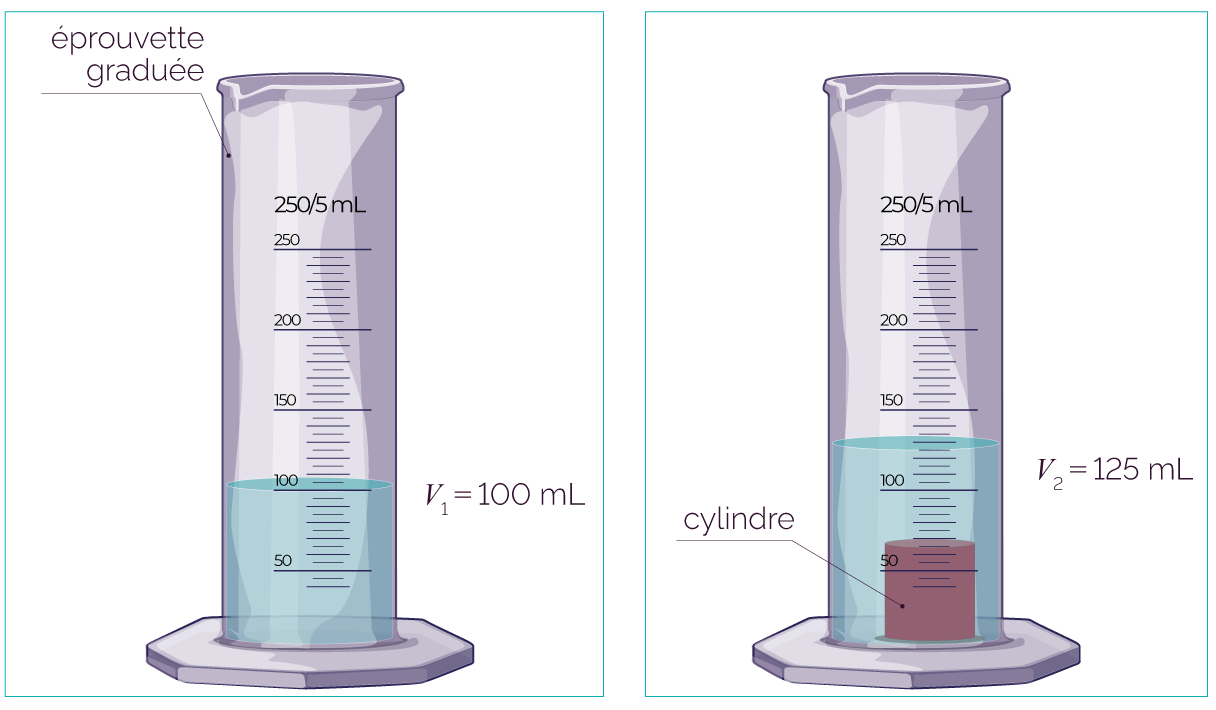
\includegraphics[width=0.7\linewidth]{eprouvette_graduee.png}
  \caption{\label{} Différence de volume}
\end{figure}

Déterminer la masse : \par
Dans le cas où le corps est solide, une balance permet facilement de trouver sa masse.

\textbf{\textcolor{blue}{Exemple}} \par 

On verse un volume \(V_1\) de 100 mL dans l'éprouvette graduée.
On plonge le corps dont on veut connaitre le volume
On lit : \(V2 = 125 mL\).

On pèse le solide : il pèse 196.5 grammes

A quel solide peut-il correspondre ?

\begin{tabular}{|l|c|c|c|c|c|c|c|}
  \hline
  Métal & Or & Argent & Cuivre & Plomb & Aluminium & Fer & Zinc \\
  \hline
  Masse volumique (en kg/L) & 19,3 & 10,5 & 8,9 & 11,3 & 2,7 & 7,9 & 7,1 \\
  \hline
  \end{tabular}


\subsection*{Détermination de la masse volumique d'un liquide}

Dans le cas où le corps étudié est liquide, la masse et le volume peuvent être facilement trouvés à l'aide d'une balance et d'une éprouvette.

Méthode

\begin{enumerate}[noitemsep]
  \item Déposer une éprouvette sur une balance.
  \item Tarer la balance à 0.
  \item Lire la masse et le volume pour calculer la masse volumique du liquide étudié.
  \begin{itemize}
    \item Remplir l'éprouvette d'un volume quelconque de liquide.
    \item Lire la masse donnée par la balance.
    \item Lire le volume en respectant la place de l’œil pour éviter les erreurs. 
    \item Calculer la masse volumique du liquide étudié
  \end{itemize}
\end{enumerate}

\begin{figure}[H]
  \centering
  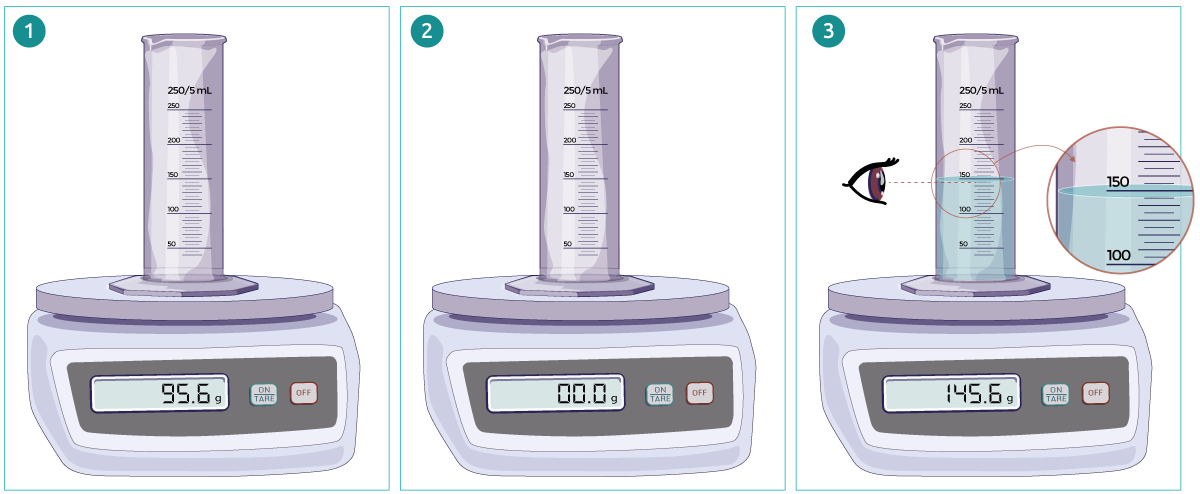
\includegraphics[width=0.7\linewidth]{eprouvette_graduee_liquide.png}
  \caption{\label{} Masse  volumique d'un liquide}
\end{figure}


\end{document}


\section*{Exercices}

Correction de l'exercice 10 Page 16
A faire chez soi : Exercice 12, 13, 16
